\begin{figure}
    \centering
    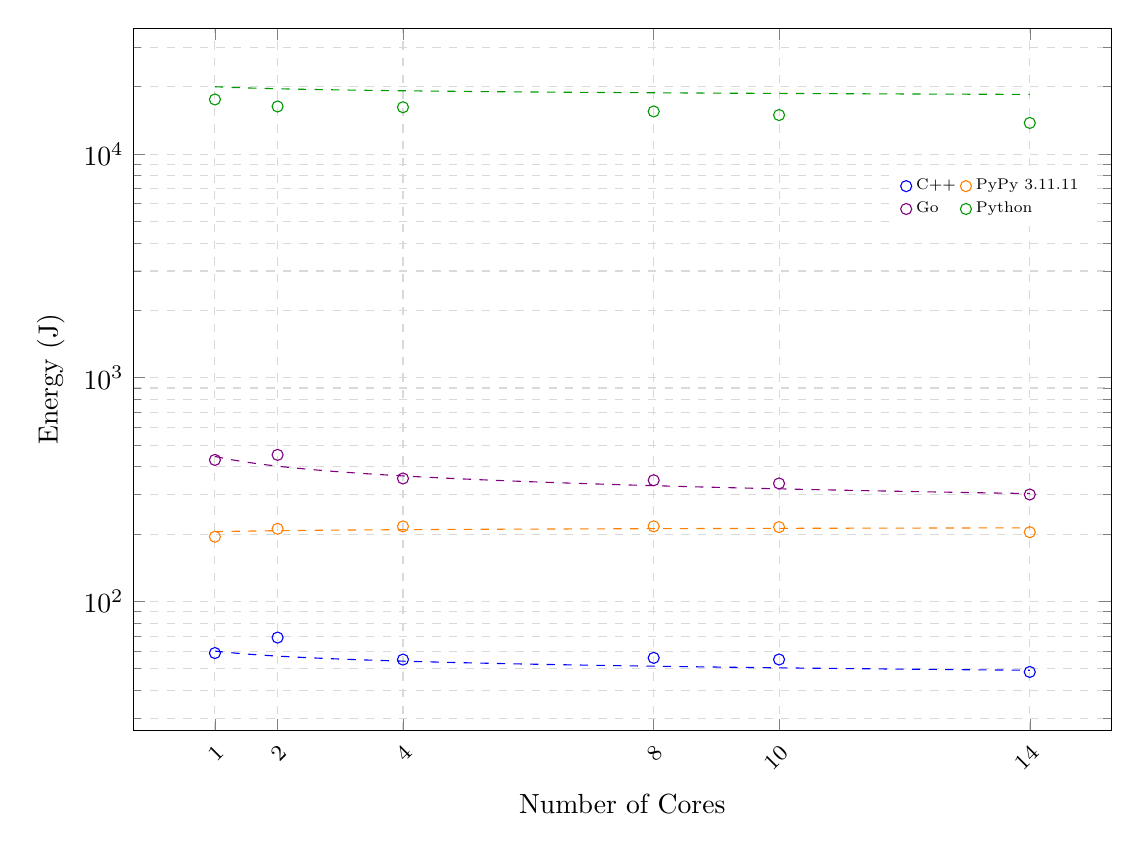
\begin{tikzpicture}
    %% Add a title for the figure
  \begin{semilogyaxis}[
      width=14cm,
        height=10.5cm,
        xlabel={Number of Cores},
        ylabel={Energy (J)},
        ymode=log,
        xmode=linear,
        grid=both,
        minor tick num=1,
        grid style={gray!30,dashed},
        xtick={1,2,4,8,10,14},
        x tick label style={
          font=\footnotesize,
          rotate=45,
          anchor=north east
        },
        legend style={
          at={(0.98,0.8)},
          anchor=north east,
          font=\scriptsize,
          nodes={scale=0.8,transform shape},
          draw=none
        },
        legend columns=2,
        transpose legend,
        legend cell align=left,
          ]
          %% C++ %%
          \addplot[
        blue,
        only marks,
        mark=o,
        mark options={draw=blue,fill=white}
          ]
          table[row sep=\\] {
        x    y      \\
        1    58.79  \\
        2    68.93  \\
        4    54.97  \\
        8    55.94  \\
        10   55.00  \\
        14   48.39  \\
          };
          \addlegendentry{C++}
          % Updated power‐law fit: y = 60.0 * x^(-0.075)
          \addplot[
        blue,
        dashed,
        forget plot,
        domain=1:14,
        samples=200
          ] {60.0 * x^(-0.075)};
          
          %% Go %%
          \addplot[
        violet,
        only marks,
        mark=o,
        mark options={draw=violet,fill=white}
          ]
          table[row sep=\\] {
        x     y       \\
        1     429.23  \\
        2     452.12  \\
        4     354.64  \\
        8     348.14  \\
        10    336.88  \\
        14    300.66  \\
          };
          \addlegendentry{Go}
          % Updated power‐law fit: y = 445 * x^(-0.145)
          \addplot[
        violet,
        dashed,
        forget plot,
        domain=1:14,
        samples=200
          ] {445 * x^(-0.145)};
          
          %% PyPy 3.11.11 %%
          \addplot[
        orange,
        only marks,
        mark=o,
        mark options={draw=orange,fill=white}
          ]
          table[row sep=\\] {
        x    y      \\
        1    194.69 \\
        2    211.21 \\
        4    216.53 \\
        8    216.60 \\
        10   214.96 \\
        14   203.92 \\
          };
          \addlegendentry{PyPy 3.11.11}
          % Updated power‐law fit: y = 205 * x^(0.015)
          \addplot[
        orange,
        dashed,
        forget plot,
        domain=1:14,
        samples=200
          ] {205 * x^(0.015)};
          
          %% Python %%
        \addplot[
        green!60!black,
        only marks,
        mark=o,
        mark options={draw=green!60!black,fill=white}
          ]
        table[row sep=\\] {
        x      y        \\
        1      17546.05 \\
        2      16322.57 \\
        4      16193.99 \\
        8      15509.12 \\
        10     14942.09 \\
        14     13777.34 \\
        };
        \addlegendentry{Python}
        % Updated power‐law fit: y = 20000 * x^(-0.030)
        \addplot[
          green!60!black,
          dashed,
          forget plot,
          domain=1:14,
          samples=200
        ] {20000 * x^(-0.030)};

  \end{semilogyaxis}
\end{tikzpicture}
    \caption{Logarithm Energy consumption of the MBP algorithm in different programming languages.}
    \label{fig:log-mbp-energy}
\end{figure}

\begin{figure}
    \centering
    
    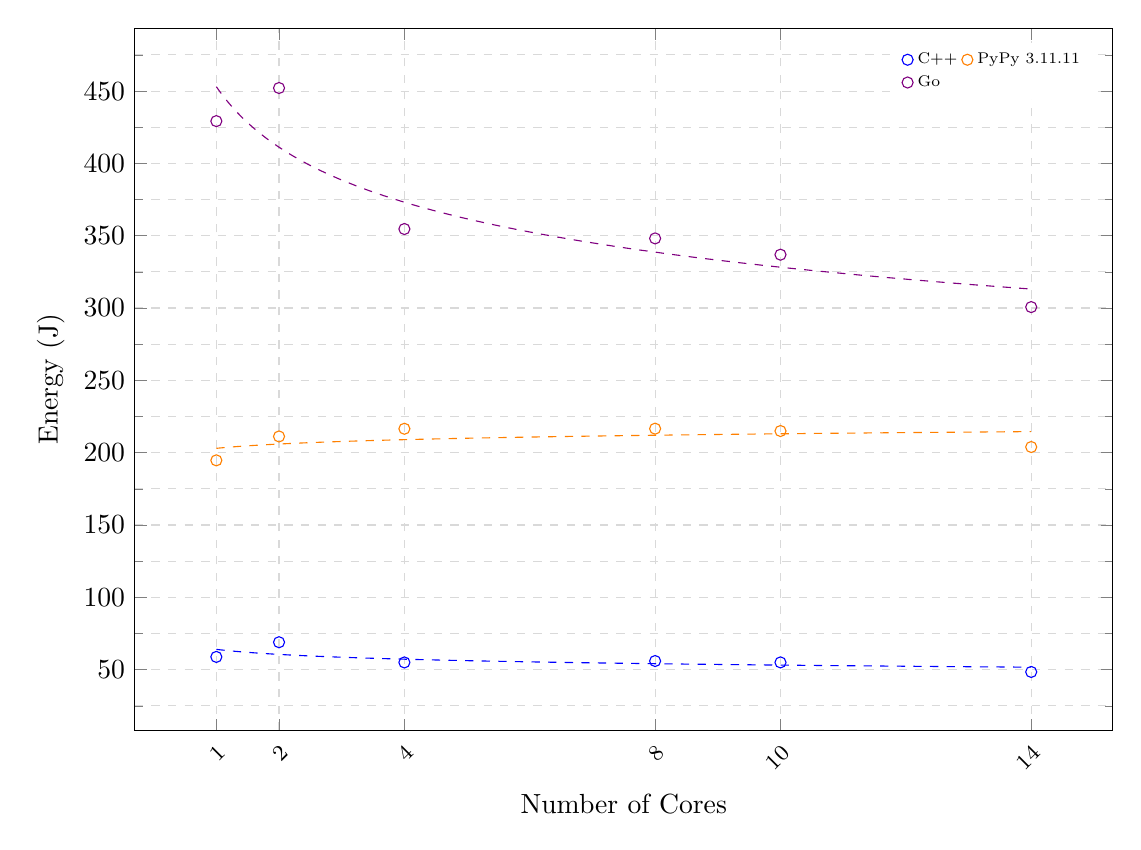
\begin{tikzpicture}
  \begin{axis}[
      width=14cm,
      height=10.5cm,
      xlabel={Number of Cores},
      ylabel={Energy (J)},
      ymode=linear,
      xmode=linear,
      grid=both,
      minor tick num=1,
      grid style={gray!30,dashed},
      xtick={1,2,4,8,10,14},
      x tick label style={
        font=\footnotesize,
        rotate=45,
        anchor=north east
      },
      legend style={
        at={(0.98,0.98)},
        anchor=north east,
        font=\scriptsize,
        nodes={scale=0.8,transform shape},
        draw=none
      },
      legend columns=2,
      transpose legend,
      legend cell align=left,
    ]
    %% C++ %%
    \addplot[
      blue,
      only marks,
      mark=o,
      mark options={draw=blue,fill=white}
    ]
    table[row sep=\\] {
      x    y      \\
      1    58.79  \\
      2    68.93  \\
      4    54.97  \\
      8    55.94  \\
      10   55.00  \\
      14   48.39  \\
    };
    \addlegendentry{C++}
    % power‐law fit: y = 64.0 * x^(–0.081)
    \addplot[
      blue,
      dashed,
      forget plot,
      domain=1:14,
      samples=200
    ] {64.0 * x^(-0.081)};

    %% Go %%
    \addplot[
      violet,
      only marks,
      mark=o,
      mark options={draw=violet,fill=white}
    ]
    table[row sep=\\] {
      x     y       \\
      1     429.23  \\
      2     452.12  \\
      4     354.64  \\
      8     348.14  \\
      10    336.88  \\
      14    300.66  \\
    };
    \addlegendentry{Go}
    % power‐law fit: y = 453 * x^(–0.140)
    \addplot[
      violet,
      dashed,
      forget plot,
      domain=1:14,
      samples=200
    ] {453 * x^(-0.140)};

    %% PyPy 3.11.11 %%
    \addplot[
      orange,
      only marks,
      mark=o,
      mark options={draw=orange,fill=white}
    ]
    table[row sep=\\] {
      x    y      \\
      1    194.69 \\
      2    211.21 \\
      4    216.53 \\
      8    216.60 \\
      10   214.96 \\
      14   203.92 \\
    };
    \addlegendentry{PyPy 3.11.11}
    % power‐law fit: y = 203 * x^(0.021)
    \addplot[
      orange,
      dashed,
      forget plot,
      domain=1:14,
      samples=200
    ] {203 * x^(0.021)};

  \end{axis}
\end{tikzpicture}

    \caption{Linear Energy consumption of the MBP algorithm in different programming languages.}
    \label{fig:linear-mbp-energy}
\end{figure}

\begin{table}
    \centering
    \begin{tabular}{lrrrr}
        \hline
        Cores & C++   & Go     & PyPy 3.11.11 & Python      \\
        \hline
        1     & 58.79  & 429.23  & 194.69       & 17,546.05   \\
        2     & 68.93  & 452.12  & 211.21       & 16,322.57   \\
        4     & 54.97  & 354.64  & 216.53       & 16,193.99   \\
        8     & 55.94  & 348.14  & 216.60       & 15,509.12   \\
        10    & 55.00  & 336.88  & 214.96       & 14,942.09   \\
        14    & 48.39  & 300.66  & 203.92       & 13,777.34   \\
        \hline
    \end{tabular}
    \caption{Power consumption by implementation and core count}
    \label{tab:mbp-power-consumption}
\end{table}